\documentclass[11pt,twoside,a4paper]{article}
\usepackage[utf8]{inputenc}
\usepackage[english,german]{babel}
\usepackage{utopia}
\usepackage[margin=1in]{geometry}
\usepackage[parfill]{parskip}
\usepackage{makeidx}
\usepackage[onehalfspacing]{setspace}
\usepackage{fancyhdr}
\usepackage{lastpage}
\usepackage{hyperref}
\usepackage{graphicx}
\renewcommand{\sffamily}{phv}

\newcommand{\titleText}{Datenbank Hotel Projekt}
\newcommand{\authorText}{Zoe Isler, Patrick Günthard}
\newcommand{\dateText}{\today}

\title{\titleText}
\author{\authorText}
\date{\dateText}

\pagestyle{fancy}
\fancyhf{}

\fancyhead[EL]{\titleText}
\fancyhead[OR]{\authorText}
\cfoot{\thepage \space von \pageref{LastPage}}

\begin{document}
	\maketitle
	\tableofcontents
	\section{Neues ERD}
	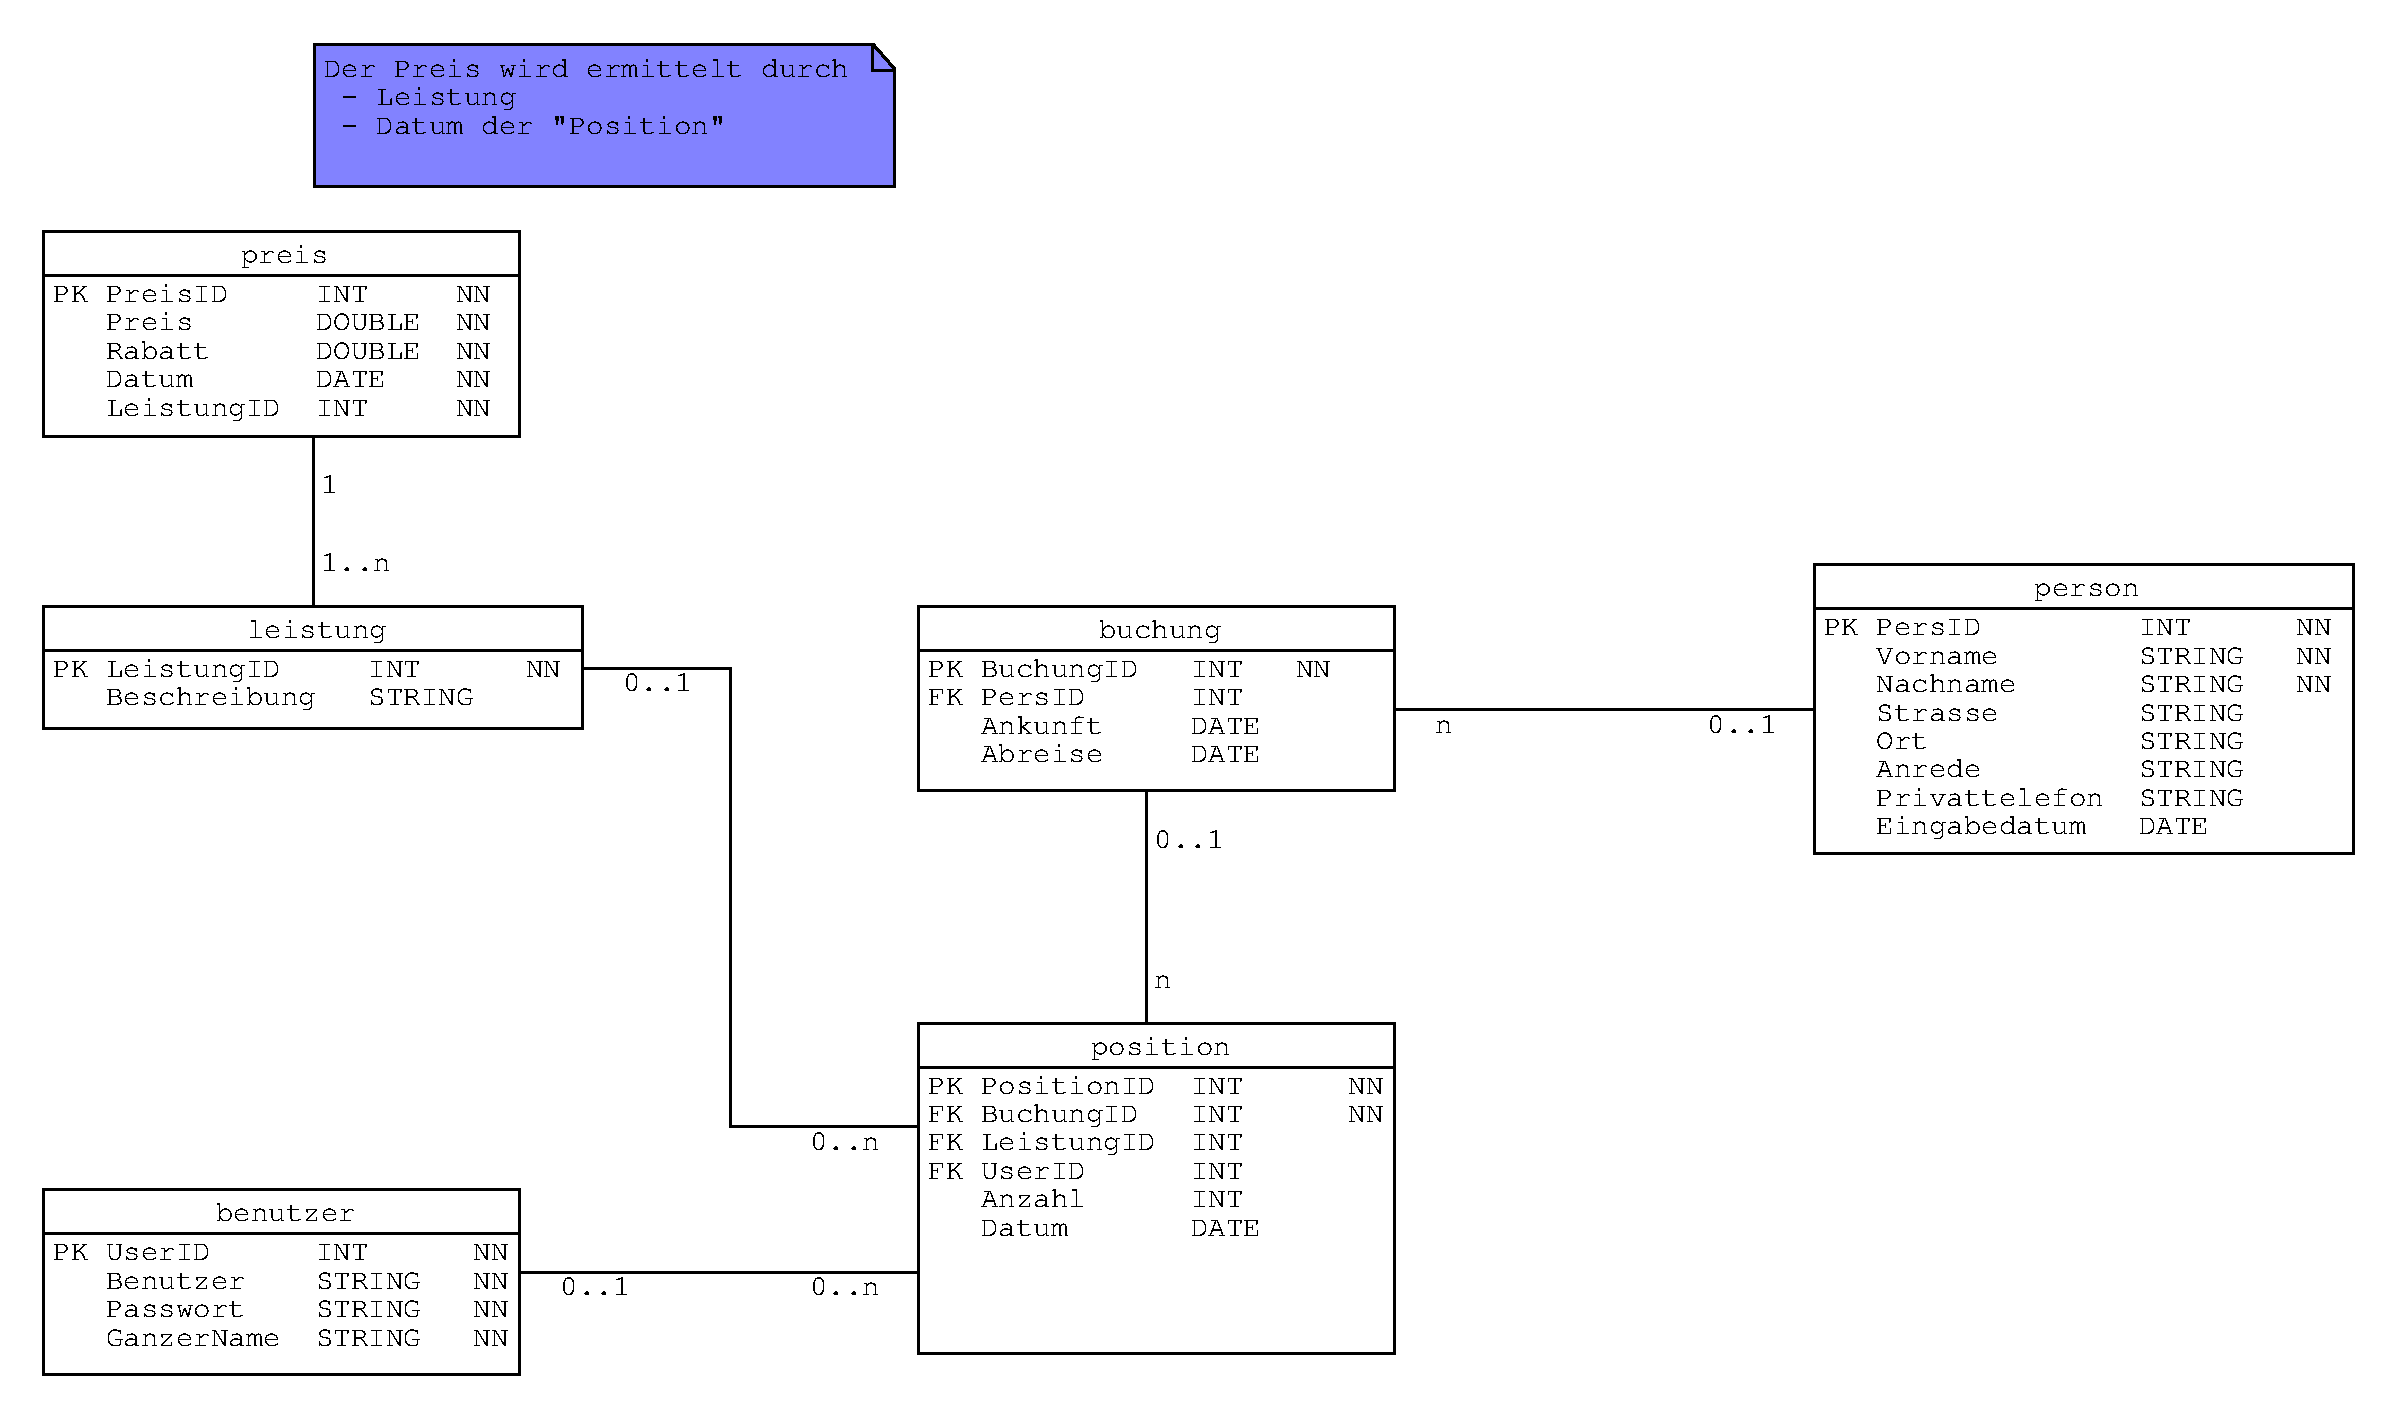
\includegraphics[width=14cm]{erd}
	\section{Änderungen}
	Es wurde eine neue Tabelle hinzugefügt: Tabelle \textit{\textbf{preis}}. [Abbildung \ref{fig:preis}]
	
	\begin{figure}
		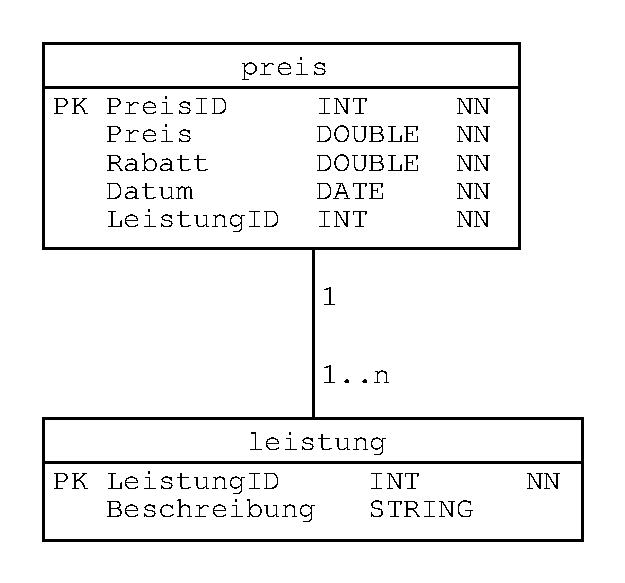
\includegraphics[width=10cm]{erd_change}
		\caption{preis \label{fig:preis}}
	\end{figure}
	
	
	Die Felder \textit{Preis} und \textit{Rabatt} wurden von der Tabelle \textit{position} nach \textit{preis} verschoben. Von [Abbildung \ref{fig:poso}] zu [Abbildung \ref{fig:posc}]
	
	\begin{figure}
		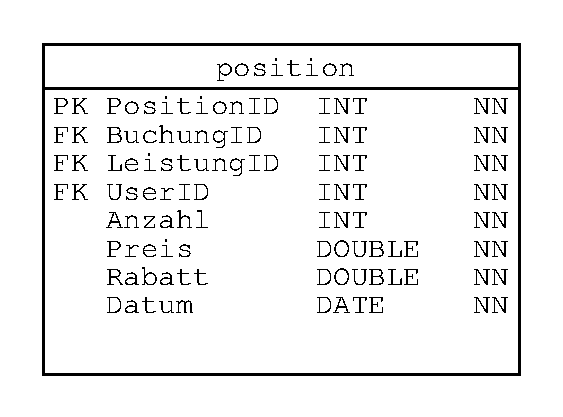
\includegraphics[width=10cm]{erd_position_orig}
		\caption{Tabelle \textit{position} \textbf{vor} der Veränderung \label{fig:poso}}
	\end{figure}
	
	\begin{figure}
		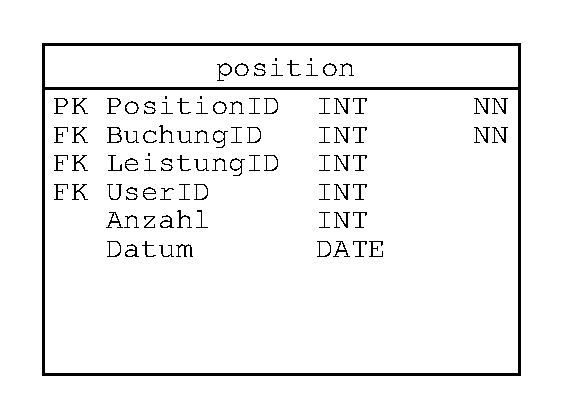
\includegraphics[width=10cm]{erd_position_change}
		\caption{Tabelle \textit{position} \textbf{nach} der Veränderung \label{fig:posc}}
	\end{figure}
\end{document}